



Die Grundlegende Idee bestand darin eine Frequenzanalyse mit Wavelets zu machen. Diese kann dann gebraucht werden um die Signale nach belieben zu manipulieren und nach wünschen anzupassen. Die Multiskalenanalyse bietet einen schnellen Rechenalgorhytmus jedoch ist er darauf konzipiert keine redundate Daten zu erzeugen. Dadurch ist die Methode für eine für eine  Durch das prinzip der Frequenzhalbierung die auf jedem sogenannten Level einer Multiskalenanalyse passiert sieht man nur alle Oktaven eines Signales. So können Frequenzen die nahe bei einander liegen nicht von einander unterschieden werden. Das ursprüngliche Signal lässt sich nach einer msa wieder verlustfrei rekonstruieren, ist jedoch zur analyse ungeeignet.\\



\subsection{Framing}
Die normale msa besitzt nur Orthonormierte Basen weshalb sie auch keine redundante Daten besitzt. Zur analyse zwecken würde es sich lohnen mehr von diesen Basen zu erzeugen und die enstehung der zusätzlichen Informationen zu verwenden. 


\begin{figure}[!ht]
	\centering
	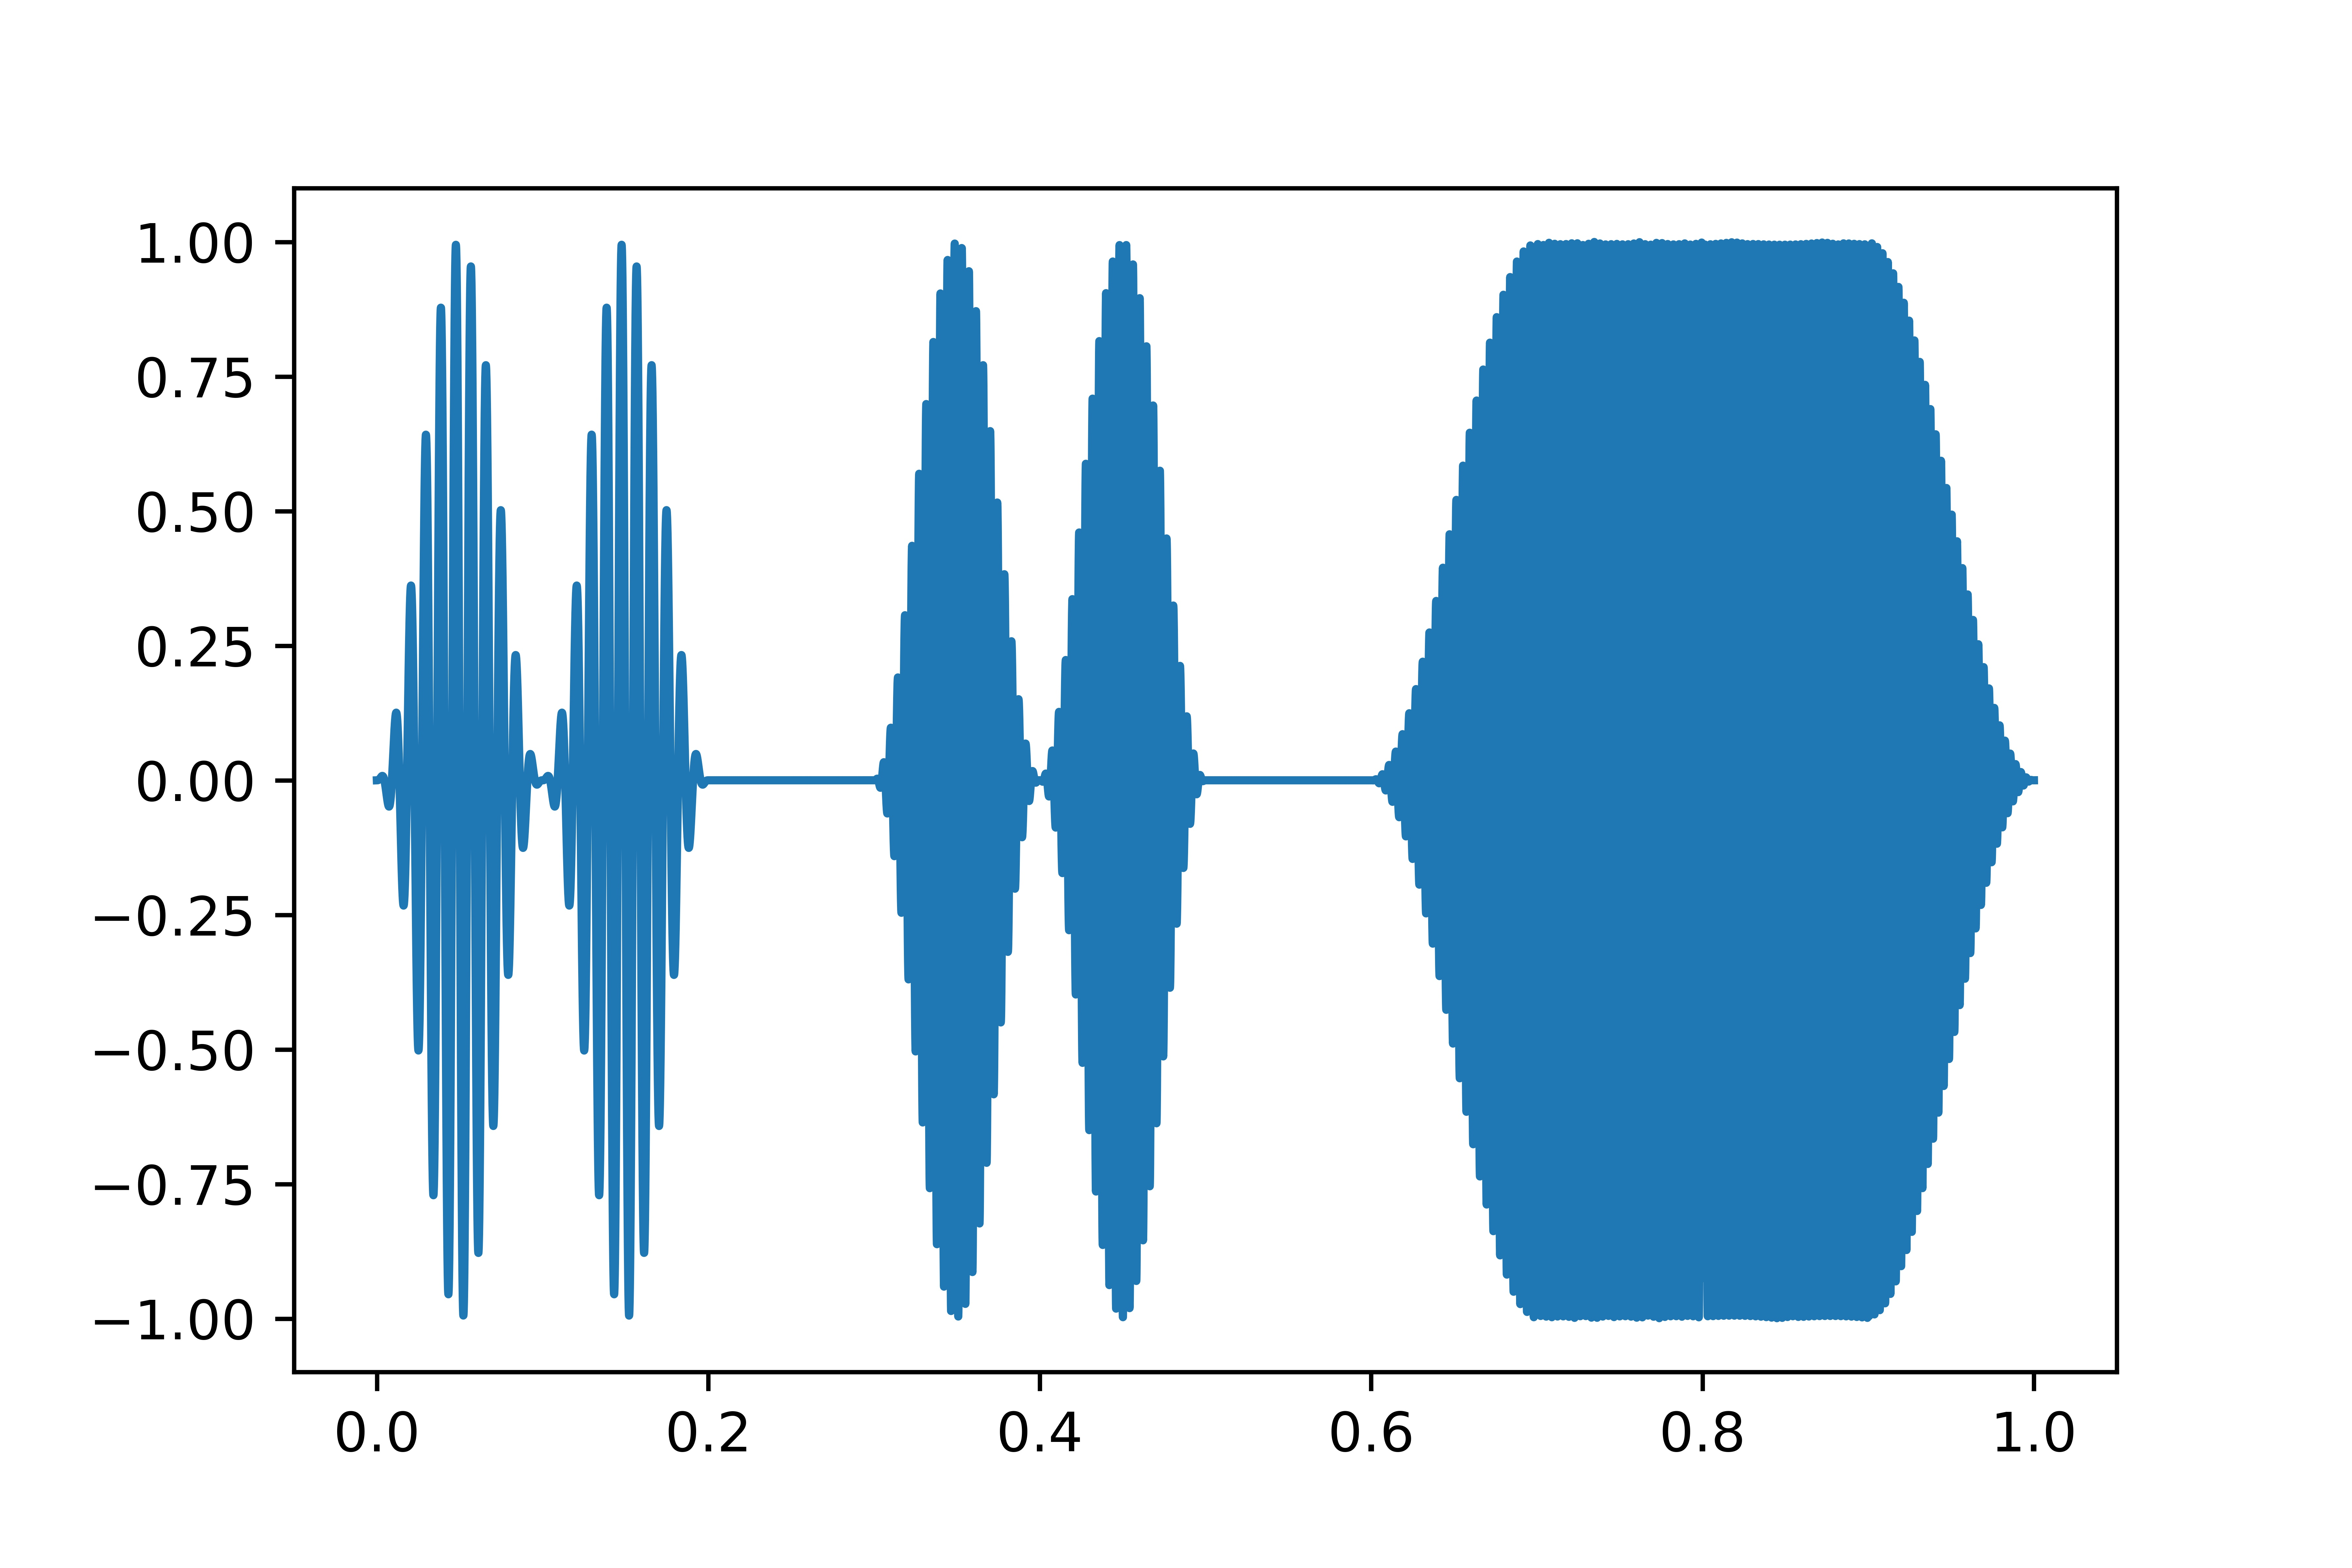
\includegraphics[width=\columnwidth]{papers/autotune/sections/frames/images/testsig.jpg}
	\captionof{figure}{Testsignal}\label{fig:frame}
	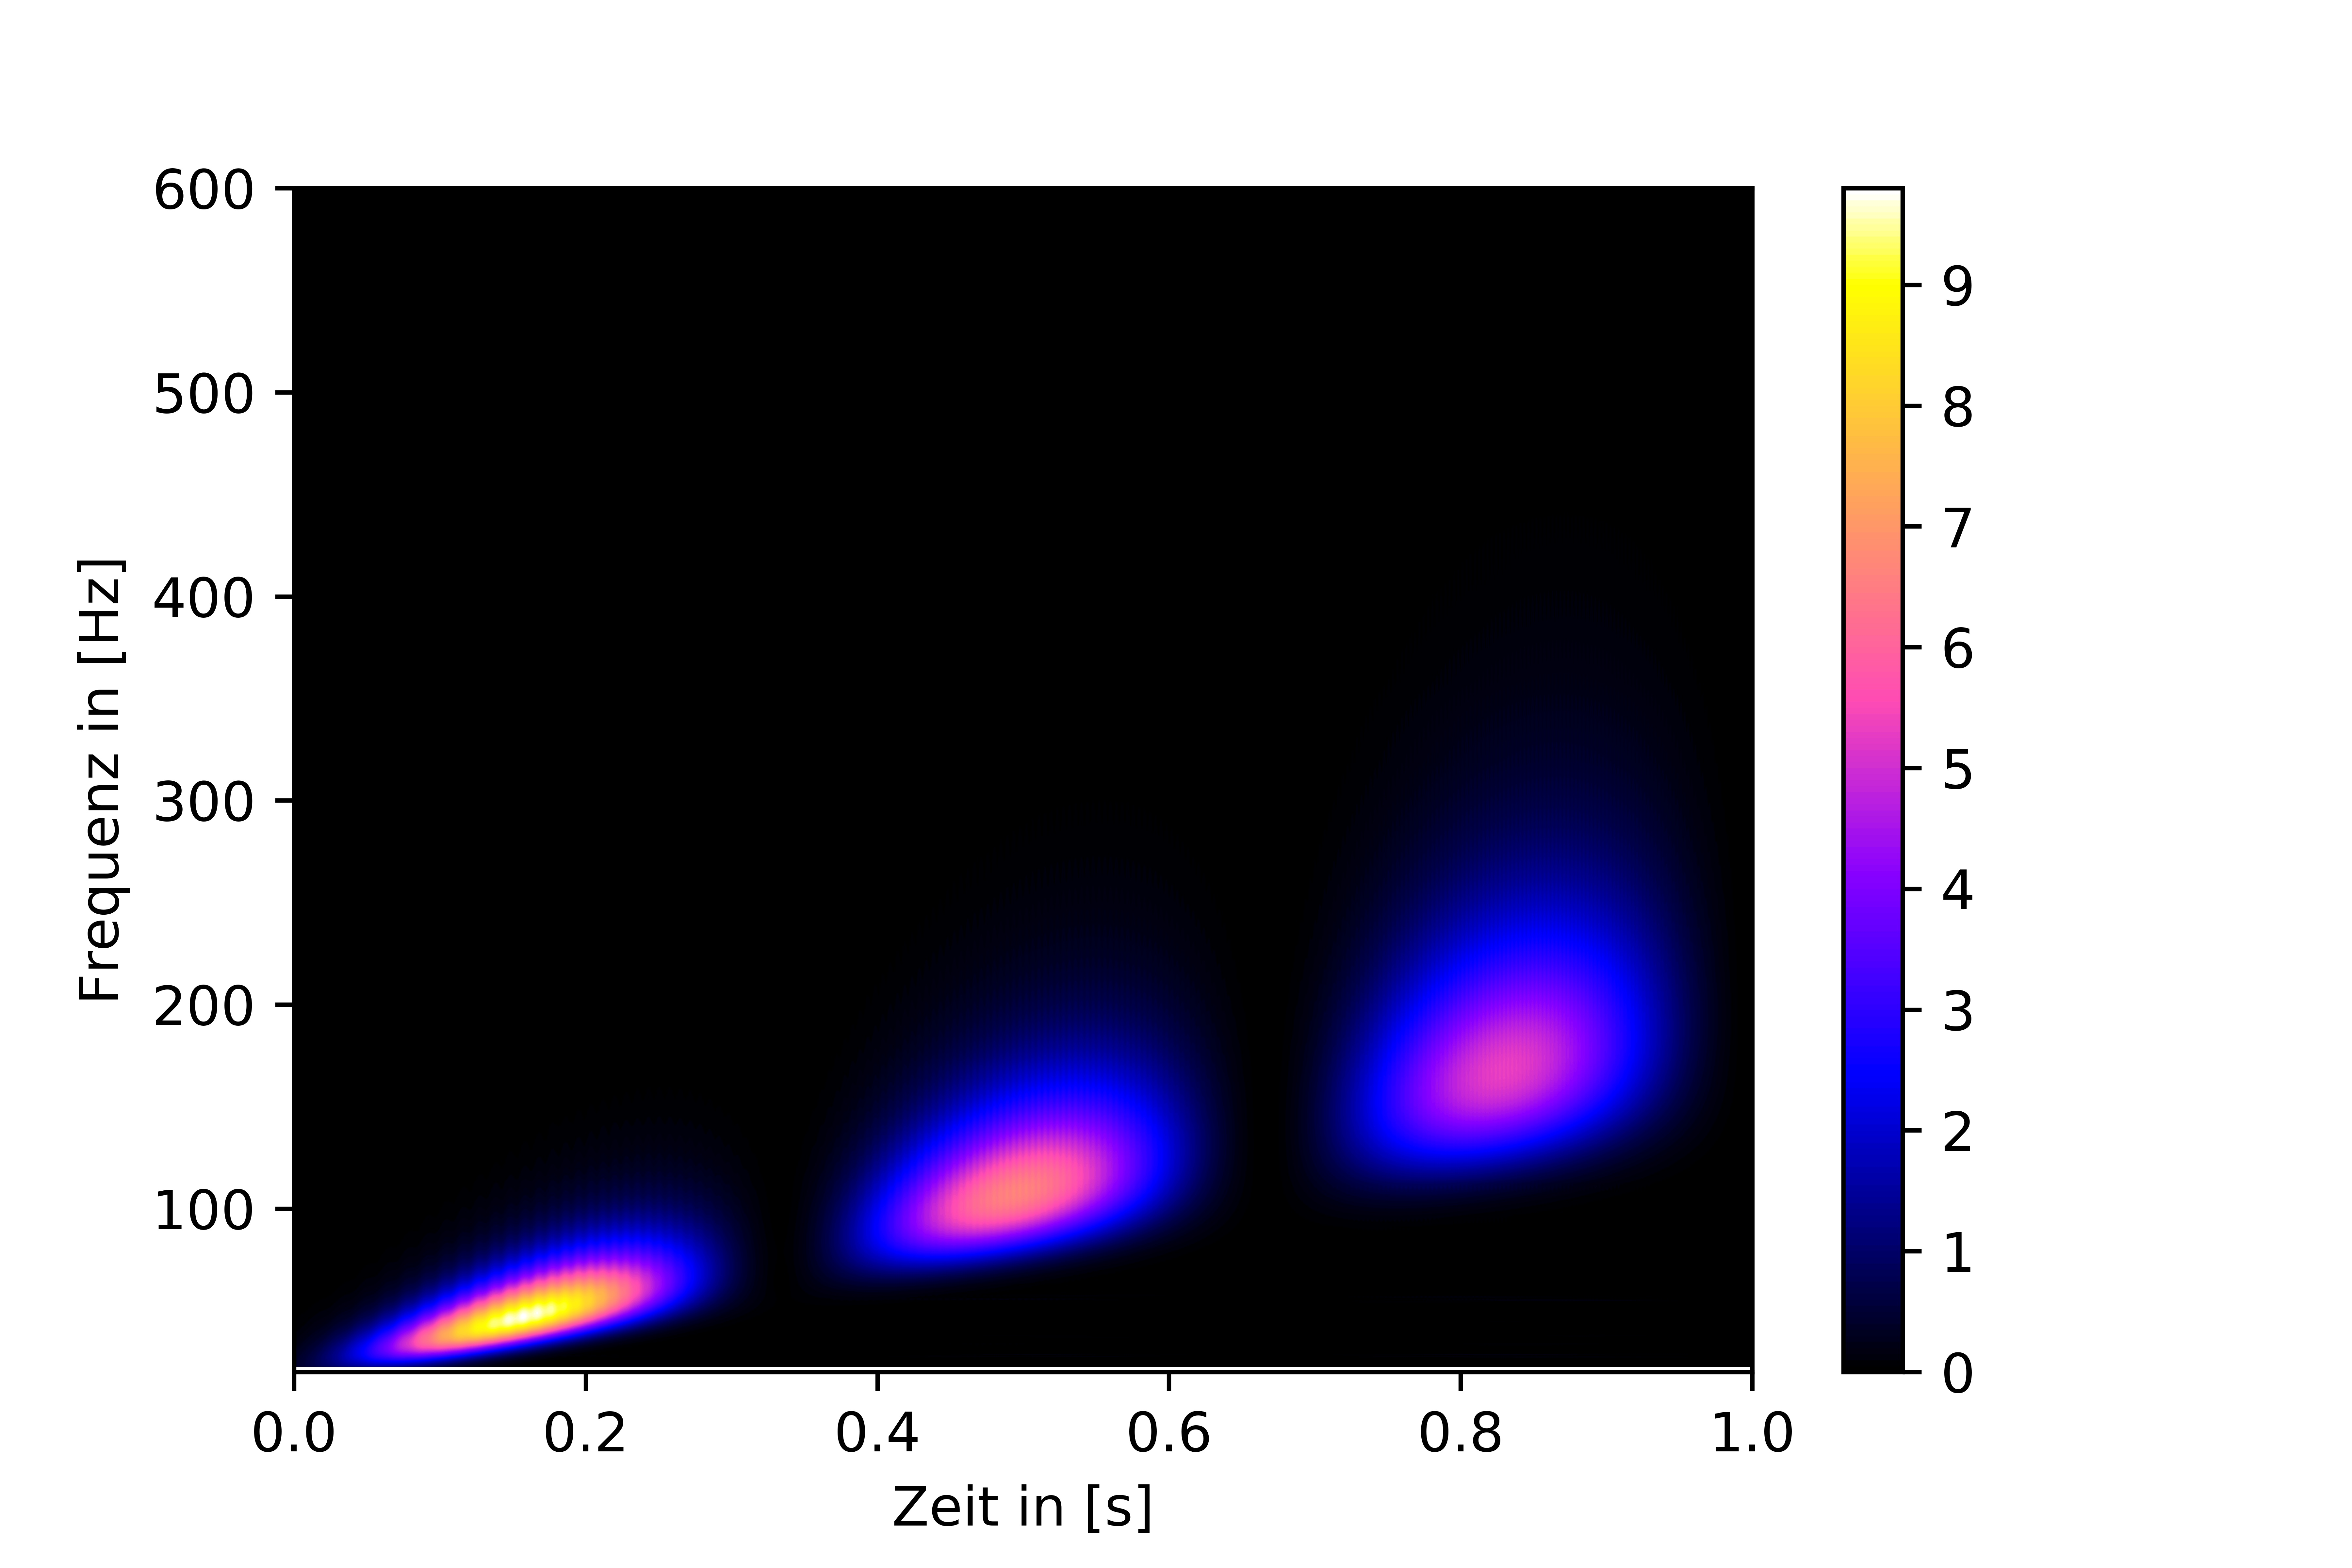
\includegraphics[width=\linewidth]{papers/autotune/sections/frames/images/sincosmcwt.jpg}
	\captionof{figure}{Dauberchi 8 cwt des Testsignales}\label{fig:stft256}
	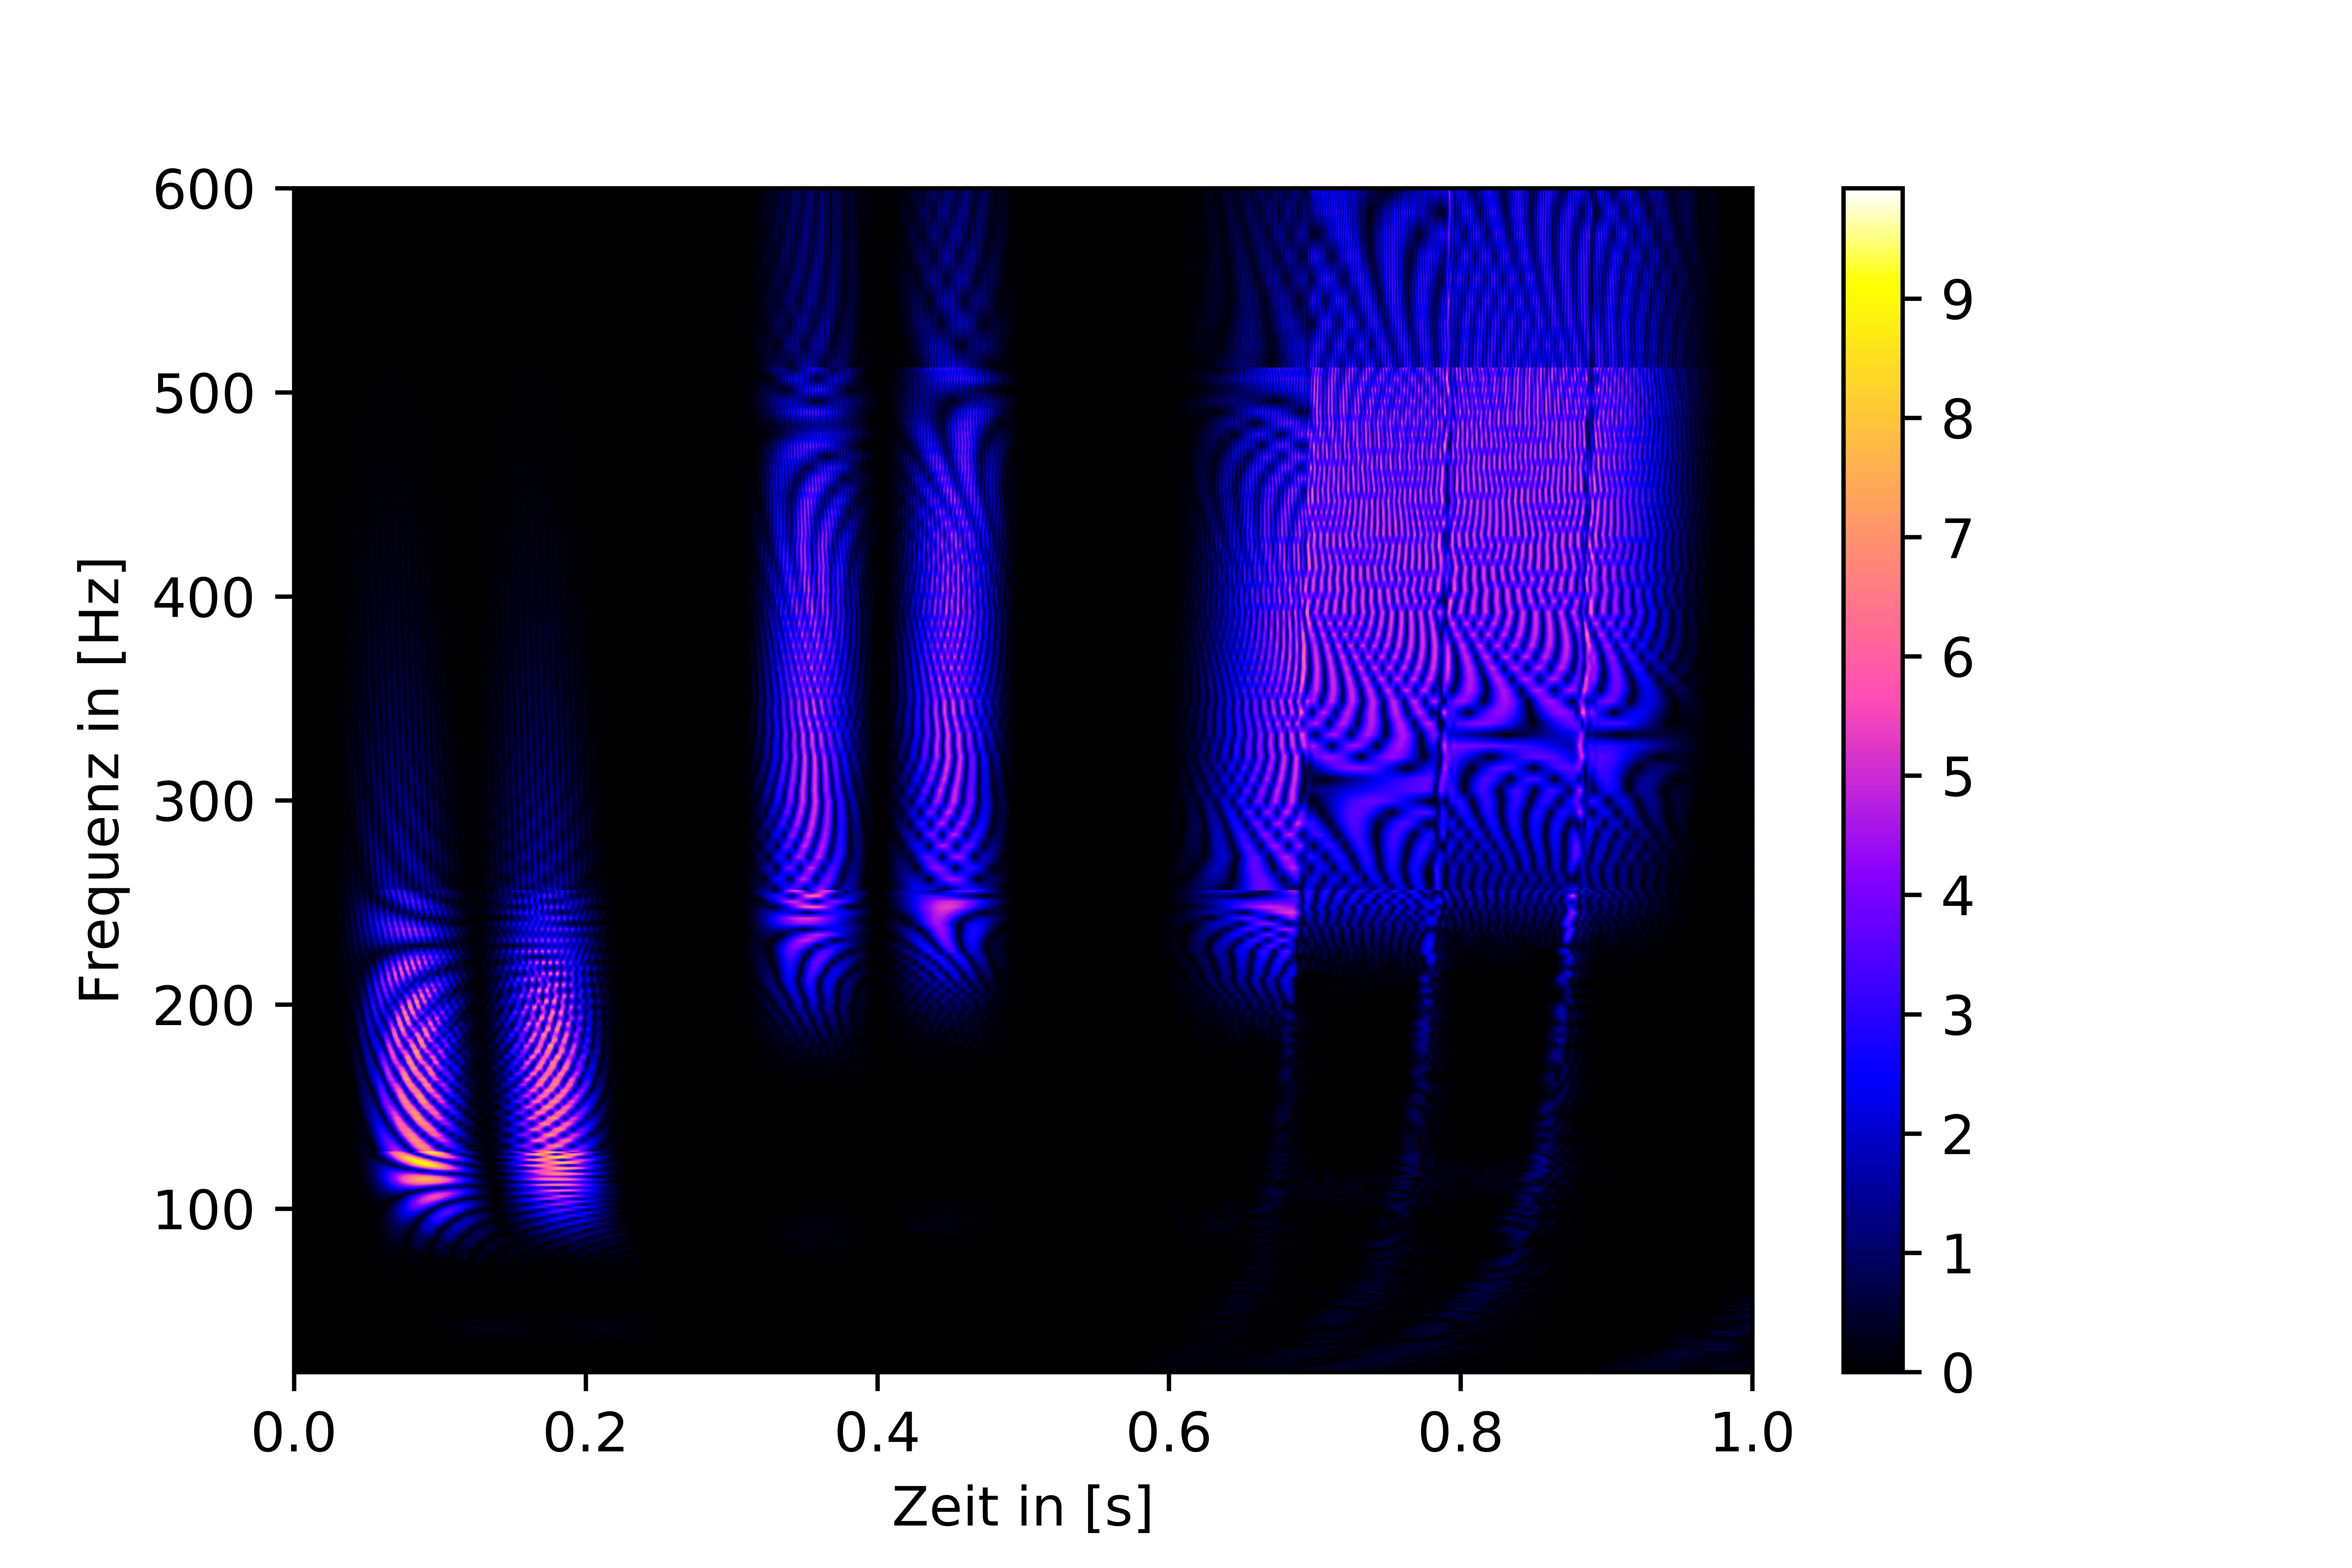
\includegraphics[width=\linewidth]{papers/autotune/sections/frames/images/sincosmdwt.jpg}   
	\captionof{figure}{Frame}\label{fig:stft1024}                        
	\caption{Vergleich der Absolutwerte von der cwt und der Frame Analyse mit 48 Basen}
	\label{fig:STFT}
\end{figure}%




Folgend der essenzielle Ausschnitt aus dem Python Code:
\begin{figure}[!ht]
	\centering
	\lstinputlisting[language=Python,firstline=1,lastline=49,numbers=left,style = mystyle]{papers/autotune/code/mdwt.py}
	\caption{Python Codeausschnitt}
	\label{fig:python-code}
\end{figure}